\subsection{QUBO}
Quadratic Unconstrained Binary Optimisation (QUBO) is an NP-hard combinatorial optimisation problem. It serves as a general mathematical description for many widely studied and relevant problems such as: \hl{Travelling Salesman Problem, Max-cut problem, Map coloring}.  In general form it is defined as:
\[f_Q(x) = \sum_{i=1}^n \sum_{j=1}^i q_{ij} x_i x_j\]
with $x_i\in\lbrace 0,1\rbrace$ for $i\in[n]$ and coefficients $q_{ij}\in\mathbb{R}$ for $1\leq j\leq i\leq n$.

An equivalent matrix notation of QUBO is:
\[ min\ y=x^\top Qx\]
where $Q\in\mathbb{R}^{n\times n}$ is the symmetric $n\times n$ matrix containing the coefficients $q_{ij}$.

In general, QUBO is a minimisation problem, but if $f(x)$ is a function to be maximised, it is sufficient to minimise $-f(x)$. By being a mathematical description of wide use, it is similar to Lenz-Ising model. Interestingly both descriptions are interchangeable.

\subsubsection{Natural QUBO formulations}
\label{subsub:natural_qubo}
Some of combinatorial problems fit QUBO "naturally" without any tricks. This is true for problems that do not have any constraints. One example of such problem is Number Partitioning. In common definition, its goal is to divide a set of numbers so the respective sums of the two resulting subsets are close to each other as possible. Given a set of numbers $S=\lbrace s_1,s_2,...,s_m\rbrace$, let $x_i=1$ if $s_i$ is assigned to set 1, $x_i=0$ otherwise. The sum for subset 1 is given as $sum_1=\sum_{i=1}^ms_ix_i$ and the sum for subset 2 is $sum_2=\sum_{i=1}^ms_i - \sum_{i=1}^ms_ix_i$. The difference:
\[diff=sum_1-sum_2=\sum_{i=1}^ms_i - 2\sum_{i=1}^ms_ix_i= c - 2\sum_{i=1}^ms_ix_i\]
Let us consider the square of the difference, hence minimum will be the optimum (0):
\[diff^2=\left(c - 2\sum_{i=1}^ms_ix_i\right)^2=c^2+4\sum_{i=1}^ms_ix_i\left(\sum_{i=1}^ms_ix_i-c\right)\]
Now we can drop constant values $c^2$ and $4$ and convert the sums into vectors and matrix:
\[min\ y =\sum_{i=1}^ms_ix_i\left(\sum_{i=1}^ms_ix_i-c\right)=
\sum_{i=1}^m s_i x_i(s_i x_i-c) + 2\sum_{i=1}^m \sum_{\substack{j=1 \\ j\ne i}}^m s_i x_i s_j x_j=
x^\top Qx\],
where $q_{ii}=s_i(s_i-c)$ and $q_{ij}=q_{ji}=s_is_j$. Elements of the $Q$ matrix diagonal correspond to $x_i^2$ terms. It is important to note that because for boolean variables $x^2=x$:
\[s_i x_i(s_i x_i-c) = s_i^2 x_i^2 - c s_i x_i = x_i^2 s_i(s_i - c)\]
Other examples of problems that naturally map to QUBO are Max-Cut Problem \hl{what else?}
\subsubsection{QUBO by reformulation}
Of course the majority of interesting problems do not map so easily to QUBO. Often, additional constraints are required which do not match the "unconstrained" description. The main idea of mapping such problems is not restricting the solution but increasing the cost of infeasible solutions by using penalties. Corresponding terms are added to the basic function. If the penalty terms reach zero, whole function becomes the original, unconstrained function. Great feature of QUBO is that it is additive in nature so ideally, the final solution will be in the intersection of minimums for all constituting terms of QUBO. Sometimes such solution does not exist and some trade-offs have to be made. An increased cost is acceptable but non-physical result is clearly not. This gradation of penalty terms is done by multiplying them with weights. More important constraint will result in a penalty term with a high weight. \autoref{tab:qubo1} presents common constraints and their corresponding penalties.

\begin{table}[h]
\begin{center}
\begin{tabular}{ l l }
 Classical constraint & Equivalent penalty\\ 
  \hline
 $x_1 + x_2 \le 1$ & $P(x_1x_2)$ \\  
 $x_1 + x_2 \ge 1$ & $P(1- x_1 - x_2 + x_1x_2)$ \\
 $x_1 + x_2 = 1$ & $P(1- x_1 - x_2 + 2x_1x_2)$ \\
 $x_1 \le x_2$ & $P(x_1 - x_1x_2)$ \\
 $x_1 + x_2 + x_3 \le 1$ & $P(x_1x_2 + x_2x_3 + x_3x_1)$ \\
 $x_1 = x_2$ & $P(x_1 + x_2 - 2x_1x_2)$ \\
\end{tabular}
\end{center}
\caption{Common constraints and their corresponding penalties.}
\label{tab:qubo1}
\end{table}

where $x_i\in\lbrace 0,1\rbrace$ and $P$ is penalty weight. Also logical constraints are possible. \autoref{tab:qubo2} presents them. When the equality is met, the penalty term is $0$. $x_3$ can be substituted with a constant value if needed.


\begin{table}[h]
\begin{center}
\begin{tabular}{ l l }
 Logical constraint & Equivalent penalty\\
  \hline 
 $NOT(x_1)=x_2$ & $P(2x_1x_2-x_1-x_2+1)$ \\  
 $AND(x_1, x_2)=x_3$ & $P(x_1x_2 - 2(x_1 + x_2)x_3 + 3x_3))$ \\
 $OR(x_1, x_2)=x_3$ & $P(x_2x_1 + (x_1+x_2)(1-2x_3)+x_3$) \\
\end{tabular}
\end{center}
\caption{Logical constraints and their corresponding penalties\cite{tanahashi_application_2019}\cite{zaman_pyqubo_2021}.}
\label{tab:qubo2}
\end{table}


For constructing more elaborate penalties, logical gates are also of use. Table \autoref{tab:qubo3} presents such gates and their corresponding penalties. Please note that $AND$ gate appeared in table \autoref{tab:qubo1}.
\begin{table}[h]
\begin{center}
\begin{tabular}{ l l }
 Logical gate & Equivalent penalty\\
 \hline
 $NOT(x_1)$ & $P(1-x_1)$ \\  
 $AND(x_1, x_2)$ & $P(x_1x_2)$ \\
 $OR(x_1, x_2)$ & $P(x_1+x_2-x_1x_2)$\\
\end{tabular}
\end{center}
\caption{Logical gates and their corresponding penalties \cite{tanahashi_application_2019}\cite{zaman_pyqubo_2021}.}
\label{tab:qubo3}
\end{table}

Now let us consider a practical example of Maximal Independent Set (equivalent to Set Packing). The task is best described as graph coloring problem: mark as many graph vertices so that no two colored vertices are connected by an edge. Let us define $x_i=1$ if vertex $i$ is colored, $x_i=0$ otherwise. The objective is:
\[max\ \sum_{i=1}^mx_i\]
with additional constraints that no two vertices sharing an edge are allowed, so penalty has to be applied if $AND(x_i, x_j)$. We can use \autoref{tab:qubo3} or \autoref{tab:qubo1} and formulate a set of constraints:
\[P\sum_{ij\in E}^m x_i x_j \]
finally, one has to remember that minimisation task should be considered, so finally:
\[min\ -\sum_{i=1}^mx_i + P\sum_{ij\in E}^m x_i x_j\]

\begin{figure}[h]
	\label{fig:graph_1}
	\caption{Simple graph with three edges.}
    \centering
    \def\svgwidth{0.25\textwidth}
    \input{graphics/graph_1.pdf_tex}
\end{figure}

For a particular graph presented in \autoref{fig:graph_1} the task becomes:
\[min\ \left[-\sum_{i=1}^4x_i + P\sum_{i=1}^3 x_i x_{i+1}\right]\]
\autoref{tab:qubo_results} contains QUBO values for all possible solutions and 3 values of penalty factor $P\in{1,2,3}$. Valid solutions (rows 1-5, 10 and 11) are unaffected by the value of $P$. This is easily explained by "switching-off" of the penalties for valid solutions. Row 12 is an interesting case: for $P=1$ is seems to be among the best solutions but that is not the case for any other value of $P$. Clearly, $P$ that is to low might not exclude invalid solutions. So should it then be much higher? Rightmost column contains solutions for $P=10$. Clearly the problem discussed earlier is solved, unfortunately other issue arises: the gap between best and second best solutions gets much smaller compared to overall range of possible values ($ \frac{1}{28}=3,6\% $). For $P=2$ the gap is $25\%$. \hl{when is it a problem? DWave 4bit precision? Is it for couplings or readout as well?}

\begin{table}
\begin{center}
\begin{tabular}{l | c c c c c c c }
row&$x1$&$x2$&$x3$&$x4$&$P=1$&$P=2$&$P=10$\\
 \hline
1&0&0&0&0&0&0&0\\ 
2&0&0&0&1&-1&-1&-1\\ 
3&0&0&1&0&-1&-1&-1\\
4&0&1&0&0&-1&-1&-1\\
5&1&0&0&0&-1&-1&-1\\ 
6&0&0&1&1&-1&0&8\\ 
7&0&1&0&1&-2&-2&-2\\ 
8&0&1&1&0&-1&0&8\\ 
9&0&1&1&1&-1&1&17\\ 
10&1&0&0&1&-2&-2&-2\\ 
11&1&0&1&0&-2&-2&-2\\ 
12&1&0&1&1&-2&-1&7\\ 
13&1&1&0&0&-1&0&8\\ 
14&1&1&0&1&-2&-1&7\\ 
15&1&1&1&0&-1&1&17\\ 
16&1&1&1&1&-1&2&26\\
\end{tabular}
\end{center}
\caption{All solution of Maximal Independent Set QUBO}
\label{tab:qubo_results}
\end{table}

\subsubsection{QUBO - graph equivalence}
\label{subsub:graph_equivalence}
Let us consider one more example: 3 binary variables $a$,$b$, $c$. Exactly one of them should be equal $1$. We can think of a constraint:
\[a+b+c=1\]
As we seek a minimization task, it is best to reformulate the constraint:
\[min(a+b+c-1)^2\]
Without this step, $a=0$, $b=0$, $c=0$ would make up the minimum, despite the fact that the original constraint is not satisfied. After expansion:
\[min(a^2+b^2+c^2+2ab+2ac+2bc-2a-2b-2c+1)\]
Note that for binary variables $x=x^2$, also a constant value increases or decreases all solution values by same amount, hence it can be omitted. Finally:
\[min(2ab+2ac+2bc-a-b-c)\]
Now let us change the notation:
\[min(-\sum_{i=1}^3x_i + 2\sum_{i=1}^3\sum_{\substack{j=1 \\ j\neq i}}^3 x_i x_j)\]
After this step it becomes clear that this is an example of QUBO. In previous example it was shown how to describe a graph problem with a QUBO, but the reverse is also possible. In fact, each QUBO describes a graph. This key property that is used by D-Wave quantum annealers - a graph is constructed in the hardware and its annealing takes place. A graph of current example is shown in \autoref{fig:dwave_triangle_graph}. $q_i$ coefficients describe node biases, $q_{ij}$ describe edge weights. Considering $i, j \in \{1,\ldots N\}$, it becomes clear that a universal hardware that allows to construct any QUBO with $N$ variables, should be a hardware chip with topology of a complete graph with $N$ nodes. With sufficiently high $N$, this becomes impossible due to enormous number of required edges. This disparity and methods for dealing with it are discussed in \autoref{sub:embedding}.

\begin{figure}
	\centering
	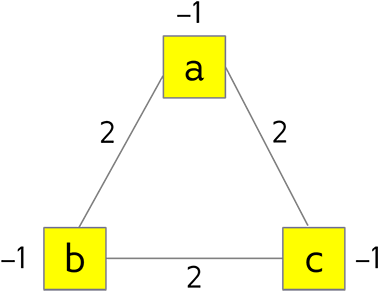
\includegraphics[width=0.4\columnwidth]{graphics/dwave_triangle_graph.png}
	\caption{A graph equivalent to QUBO describing three binary variables, where only one should be equal $1$ (true) \cite{d-wave_inc_d-wave_2022}.}
    \label{fig:dwave_triangle_graph}
\end{figure}

There of course are many cases that do not fit natural QUBO formulation discussed in \autoref{subsub:Natural_QUBO} nor are required penalties formulated as discussed in this section. For such cases a more general method is available. Please refer to \cite{glover_quantum_2019} for detailed explanation. It is also possible to use dedicated software libraries as discussed in \autoref{sub:qubo_tools}.